% EPC flow charts
% Author: Fabian Schuh
\documentclass[11pt,a4paper]{article}

\usepackage{pgf}
\usepackage{tikz}
\usepackage[utf8]{inputenc}
\usetikzlibrary{arrows,automata}
\usetikzlibrary{positioning}


\tikzset{
    state/.style={
           rectangle,
           rounded corners,
           draw=black, very thick,
           minimum height=2em,
           inner sep=2pt,
           text centered,
           },
}

\begin{document}

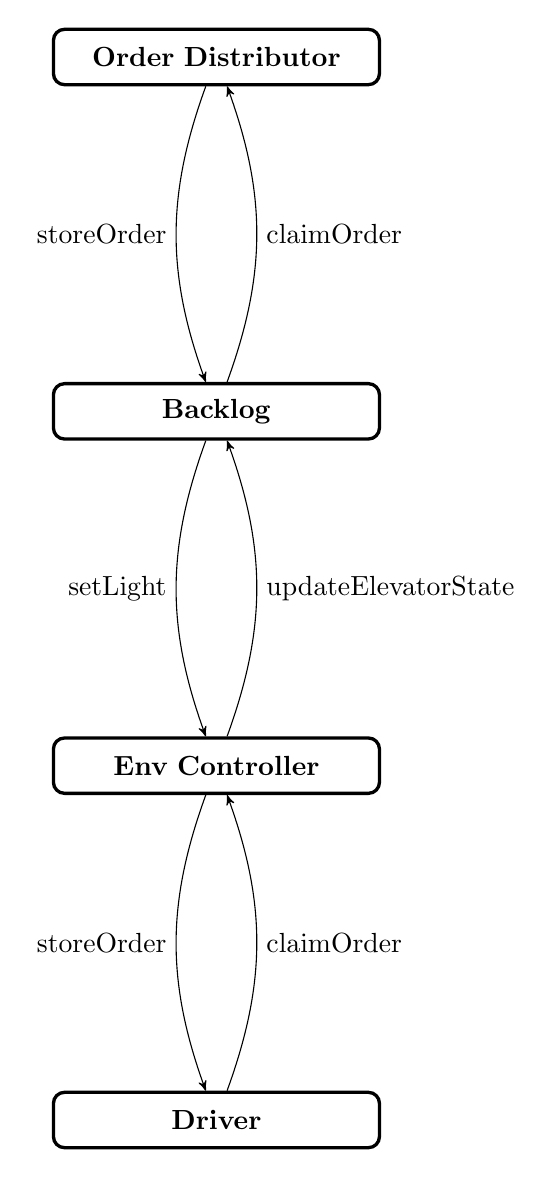
\begin{tikzpicture}[->,>=stealth']

 % Position of Env Controller 
 % Use previously defined 'state' as layout (see above)
 % use tabular for content to get columns/rows
 % parbox to limit width of the listing
 \node[state,text width=4cm] (Env Controller) 
 {\textbf{Env Controller}};

 \node[state,       % layout (defined above)
  text width=4cm,   % max text width      
  above of=Env Controller,   
  node distance=4.5cm,  
  anchor=center] (Backlog)  % posistion relative to the center of the 'box'
  {\textbf{Backlog}};
 
 % STATE Communication
 \node[state,
  above of=Backlog,
  node distance=4.5cm,
  anchor=center,
  text width=4cm] (Communication) 
 {\textbf{Order Distributor}};

 \node[state,
  below of=Env Controller,
  node distance=4.5cm,
  anchor=center,
  text width=4cm] (Driver) 
 {\textbf{Driver}};

 
 % draw the paths and and print some Text below/above the graph
 \draw[<-] (Env Controller) edge[bend left=20] node[pos=0.5,left]{setLight} (Backlog);
 \draw[->](Env Controller) edge[bend right=20] node[pos=0.5,right]{updateElevatorState} (Backlog);

 \draw[->](Communication) edge[bend right=20] node[pos=0.5,left]{storeOrder} (Backlog);
 \draw[<-](Communication) edge[bend left=20] node[pos=0.5,right]{claimOrder} (Backlog);

 \draw[->](Env Controller) edge[bend right=20] node[pos=0.5,left]{storeOrder} (Driver);
 \draw[<-](Env Controller) edge[bend left=20] node[pos=0.5,right]{claimOrder} (Driver);

\end{tikzpicture}
\end{document}